\documentclass{beamer}
\usetheme{Madrid}

\usepackage{amsmath, amssymb, amsthm}
\usepackage{graphicx}
\usepackage{listings}
\usepackage{gensymb}
\usepackage{minted}
\usemintedstyle{friendly}
\definecolor{bg}{rgb}{0.95,0.95,0.95}
\usepackage[utf8]{inputenc}
\usepackage{hyperref}
\usepackage{gvv}\begin{document}
\title{DISCRETE 1-1.5-8}
\author{EE24BTECH11029 - J.SHRETHAN REDDY$^{*}$}
\date{}
\frame{\titlepage}

\begin{frame}
\frametitle{Question}
Find the ratio in which $P\brak{4,5}$ divides the line segment joining $A\brak{2,3}$ and $B\brak{7,8}$
\end{frame}
\begin{frame}{allowframebreaks}
\frametitle{Solution: Table}
\begin{table}[h!!]
    \centering
    \begin{tabular}{|c|c|c|}
\hline
\textbf{points}& \textbf{description}& \textbf{formula}
\\\hline
$A\brak{2,3}$&one end of line segment&$-$
\\\hline
$B\brak{7,8}$&another end of line segment&$-$
\\\hline
$P\brak{4,5}$&divides $A$ and $B$ in the ratio $k:1$&$P=\frac{A+kB}{k+1}$
\\\hline
\end{tabular}
    \caption{Variables Used}
    \label{tab 10.5.4.5}
\end{table}
\end{frame}
\begin{frame}
\frametitle{Theory}
\begin{align}
 P&=\frac{\vec{A}}{k+1}+\frac{k\vec{B}}{k+1}\\
\label{eq:section_formula}
\implies p&=\myvec{\Vec{A}&\Vec{B}}\myvec{\frac{1}{k+1}\\\frac{k}{k+1}}
\end{align}
\end{frame}
\begin{frame}
\frametitle{Theory}
\begin{align}
 from \eqref{eq:section_formula}\\
 \implies\myvec{4\\5}&=\myvec{2&7\\3&8}\myvec{\frac{1}{k+1}\\\frac{k}{k+1}}\\
\implies \myvec{4\\5}&=\myvec{\frac{2}{k+1}+\frac{7k}{k+1}\\\frac{3}{k+1}+\frac{8k}{k+1}}\\
\implies 4&=\frac{2+7k}{k+1}\\
\implies 4k+4&=2+7k\\
3k&=2\\
k&=\frac{2}{3}\\
\end{align}
\end{frame}

\begin{frame}
\frametitle{Theory}
\begin{align}   
k\colon1&=\frac{2}{3}\colon1
\end{align}
\end{frame}

\begin{frame}[fragile]
\frametitle{C-Code}
\begin{minted}[bgcolor=bg, linenos, fontsize=\small, breaklines]{c}

#include <stdio.h>
#include <stdlib.h>
#include <math.h>
#include "libs/matfun.h"
#include "libs/geofun.h"

int main() {

    int x2 = 2, y2 = 3;
    int x3 = 7, y3 = 8;
    int x1 = 4, y1 = 5;

    int m = x1 - x2; 
    int n = x3 - x1; 

    FILE *file = fopen("output.txt", "w");

    
\end{minted}
\end{frame}
\begin{frame}[fragile]
\frametitle{C-Code}
\begin{minted}[bgcolor=bg, linenos, fontsize=\small, breaklines]{c}

    if (file == NULL) 
    {
        printf("Error opening file.\n");
        return 1;
    }
    if ((y1 - y2) * n != (y3 - y1) * m) 
    {
        fprintf(file, "The point does not divide the line segment in a constant ratio.\n");
    } else {
        fprintf(file, "%d:%d\n", m, n);
    }

    fclose(file);

    return 0;
}
\end{minted}
\end{frame}
\begin{frame}
\frametitle{c code output}
$2:3$
\end{frame}
\begin{frame}[fragile]
  \frametitle{Python Code }

\begin{minted}[bgcolor=bg, linenos, fontsize=\small, breaklines]{python}

import sys  # for path to external scripts
sys.path.insert(0, '/home/jsr/Desktop/matgeo/codes/CoordGeo')  # path to my scripts
import numpy as np
import matplotlib.pyplot as plt

# Local imports (assuming these scripts exist and are correct)
from line.funcs import *
from triangle.funcs import *
from conics.funcs import circ_gen

def read_ratio_from_file(filename):
    with open(filename, 'r') as file:
        line = file.readline().strip() 
        a_str, b_str = line.split(':')  # Split the line by ':'
        a, b = int(a_str), int(b_str)   
    return b / a  
\end{minted}
\end{frame}
\begin{frame}[fragile]
  \frametitle{Python Code }

\begin{minted}[bgcolor=bg, linenos, fontsize=\small, breaklines]{python}
# Load ratio from file
filename = 'output.txt'
n = read_ratio_from_file(filename)

# Given points
A = np.array(([2,3])).reshape(-1,1)
B = np.array(([7,8])).reshape(-1,1)

# Point
P = (B + n * A) / (1 + n)  # calculating the coordinate points of P

# Generating line AB
x_AB = line_gen(A, B)

# Plotting line AB
plt.plot(x_AB[0,:], x_AB[1,:], label='$AB$')
\end{minted}
\end{frame}
\begin{frame}[fragile]
  \frametitle{Python Code }

\begin{minted}[bgcolor=bg, linenos, fontsize=\small, breaklines]{python}
# Labeling the coordinates
tri_coords = np.block([[A, B, P]])
plt.scatter(tri_coords[0,:], tri_coords[1,:])
vert_labels = ['A','B','P']
for i, txt in enumerate(vert_labels):
    plt.annotate(f'{txt}\n({tri_coords[0,i]:.0f}, {tri_coords[1,i]:.0f})',
                 (tri_coords[0,i], tri_coords[1,i]), # Point to label
                 textcoords="offset points", # Position of text
                 xytext=(20,-10), # Offset from point
                 ha='center') # Horizontal alignment

\end{minted}
\end{frame}
\begin{frame}[fragile]
  \frametitle{Python Code }

\begin{minted}[bgcolor=bg, linenos, fontsize=\small, breaklines]{python}
# Modify axes visibility
ax = plt.gca()
ax.spines['left'].set_visible(False)
ax.spines['right'].set_visible(False)
ax.spines['top'].set_visible(False)
ax.spines['bottom'].set_visible(False)

plt.legend(loc='best')
plt.grid() 
plt.axis('equal')

# Save and display plot
plt.savefig('/home/jsr/Desktop/shrethan/presentation/fig/fig.png')
plt.show()
\end{minted}
\end{frame}
\begin{frame}
\frametitle{Figure}
\begin{figure}
    \centering
    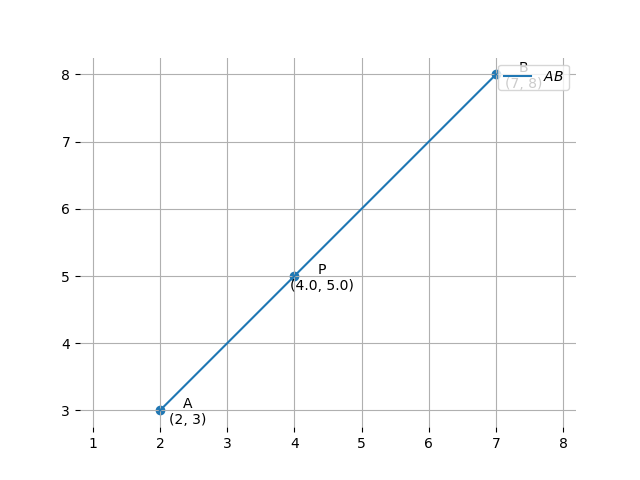
\includegraphics[width=0.7\linewidth]{fig/fig.png}
    \caption{P divides A and B in the ratio $2:3$}
    \label{fig:enter-label}
\end{figure}
\end{frame}
\end{document}
